\subsubsection{Point Mutation}
\label{sec:keen:gp:op:mutation:point}

  In the realm of Genetic Programming (GP), the concept of mutating program trees is pivotal for enhancing genetic diversity within a population. Point Mutation is one such operator, aiming to introduce slight perturbations in a program's structure, while ensuring its syntactic and semantic integrity.

  \begin{definition}[Point Mutation]
    The \textit{point mutation} operator selects a random node from a program tree and seeks another node with the same arity (number of child nodes). Once found, the original node is replaced by the new node, generating a variant of the original program tree, yet retaining its overall structure.

    Formally speaking, the operator can be expressed as:

    \begin{equation}
      X_{point}: \mathbb{P} \times [0,\, 1] \times [0,\, 1] \to \mathbb{P};\;
        (P,\, \mu_\textbf{c},\, \mu_\textbf{g}) 
        \mapsto X_{point}(P,\, \mu_\textbf{c},\, \mu_\textbf{g})
    \end{equation}

    where:

    \begin{itemize}
      \item \(P\): A population of program trees.
      \item \(\mu_\textbf{c}\): Probability of a chromosome undergoing mutation.
      \item \(\mu_\textbf{g}\): Likelihood of a gene being selected for mutation.
    \end{itemize}
  \end{definition}

  The Point Mutation operator's implementation in \textit{Keen} is straightforward. It follows a four-step process:

  \begin{code}{
    Illustration of Point Mutation in \textit{Keen}
  }{label=lst:keen:gp:op:mutation:point}{kotlin}
    val original = random node from program tree
    val replacements = nodes with same arity as original
    val replacement = random node from replacements
    val mutated = program tree with original replaced by replacement
  \end{code}

  The crux of the Point Mutation operator in the context of the \textit{Keen} 
  framework is its ability to maintain the structural coherency of program 
  trees while introducing genetic variance. 

  \begin{remark}
    Ensuring that the replacement node has the same arity is crucial. This 
    stipulation guarantees that the resulting mutated tree remains valid 
    concerning its original structure. Such an approach aids in circumventing 
    potential runtime errors or semantic misinterpretations, which could be 
    detrimental to the evolutionary process.
  \end{remark}

  The Point Mutation operator's inherent simplicity belies its effectiveness. By 
  focusing on minute alterations, it provides a balance between maintaining the 
  quality of well-performing solutions and exploring new areas of the solution 
  space.

  An illustration of the Point Mutation operator's operation is presented in
  \vref{fig:keen:gp:op:mutation:point}.

  \begin{figure}[ht!]
    \centering
    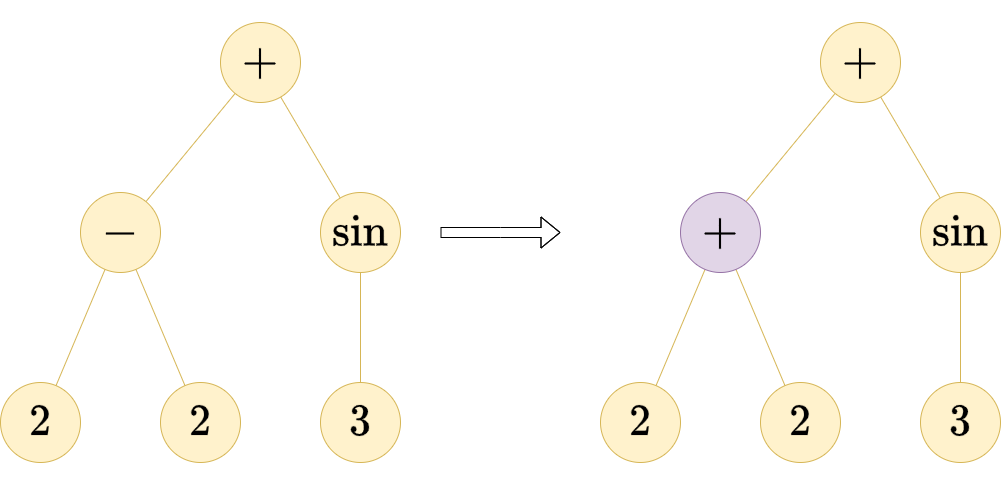
\includegraphics[width=0.5\textwidth]{img/keen/Point mutation.png}
    \caption{
      The figure depicts the Point Mutation operator's operation on a program 
      tree. The operator selects a random node from the tree and replaces it 
      with another node of the same arity. The resulting tree is a variant of 
      the original, yet it retains its overall structure.
    }
    \label{fig:keen:gp:op:mutation:point}
  \end{figure}
  